\section{Estimating the vertical model on simulated data}\label{sec:C-vertical}

The vertical model of product differentiation lets consumers differ along a single dimension, their sensitivity to
price. Every consumer ranks the products by quality in the same way, and products compete only with their neighbours
on the price ladder. These restrictions make the model easy to invert and to estimate. They also determine its
elasticities and markups almost entirely. This problem is the first of three that estimate demand on the simulated
market of \cref{sec:C-simulate}, which was generated by a random coefficients logit. Here we estimate the vertical
model. Since we know the truth, we can see exactly what the single taste
dimension does to substitution patterns, markups and recovered costs. The theory behind the model is in
\cref{sec:06-vertical}. Here we work through estimation in full.

\subsection{Statement}

The data are the 654 product-market observations of the simulated market of \cref{sec:C-simulate}. There are
$T = 100$ independent markets, and market $t$ offers $J_t$ of ten products, between 4 and 9. For each observation the
econometrician sees the price $p_{jt}$, the realized share $s_{jt} = \frac{q_{jt}}{M_t}$ and the market size $M_t$. The realized share is the $\hat s_{jt}$
of \eqref{eq:C-realized}, written without the hat in this problem and the next. The
econometrician also sees the characteristics $x_{jt} = (1, x^{sug}_{jt}, x^{org}_{jt})$ (a constant, sugar content and an organic
indicator), the price of milk $w_{jt}$ and the owner of the product. Characteristics, milk prices and owners are fixed by
product (\cref{tab:C-products}). The outside share $s_{0t} = 1 - \sum_{j} s_{jt}$ lies between 0.788 and 0.948 across
markets. The econometrician does not know how the data were generated and maintains the following assumptions.

\begin{assumption}\label{ass:C-est}
\begin{enumerate}[label=(\roman*)]
  \item Markets are independent of one another.
  \item The characteristics $x_{jt}$ and the cost shifter $w_{jt}$ are fixed (exogenous).
  \item The demand unobservable $\xi_{jt}$ and the cost unobservable $\omega_{jt}$ are independent of each other and of
  $(x_{jt}, w_{jt})$.
  \item Marginal cost is $mc_{jt} = x_{jt}\gamma_1 + \gamma_2 w_{jt} + \omega_{jt}$.
\end{enumerate}
\end{assumption}

Consumer $i$ in market $t$ obtains utility
\begin{equation}\label{eq:C-vutility}
  u_{ijt} = \delta^v_{jt} - \nu_i p_{jt}, \qquad \delta^v_{jt} = x_{jt}\beta^v + \xi_{jt},
\end{equation}
from product $j$ and $u_{i0t} = 0$ from the outside good, whose quality and price are normalized to zero. Here
$\delta^v_{jt}$ is the \emph{quality} of product $j$ in market $t$. The taste $\nu_i \ge 0$ is drawn from a continuous and
strictly increasing distribution function $F$ on $[0, \infty)$ with $F(0) = 0$ and density $f$. There is no idiosyncratic
taste shock.

\begin{enumerate}[label=(\alph*)]
  \item Derive $\delta^v_{jt}$ as a function of the prices and shares in market $t$, the market size $M_t$ and the
  inverse $F^{-1}$.
  \item Let $F(\nu) = 1 - e^{-\lambda\nu}$. Write an estimable equation for the qualities. Is $\lambda$ identified? Give
  the economic intuition. Normalize $\lambda = 1$, estimate $\beta^v$ with standard errors and discuss the fit.
  \item Keep $\lambda = 1$. Derive the marginal cost equation under (i) marginal-cost pricing and (ii) multi-product
  Bertrand-Nash pricing. Estimate $(\gamma_1, \gamma_2)$ under each conduct assumption, and explain why demand and supply
  can be estimated separately without loss of efficiency.
  \item Compute the matrix of own- and cross-price elasticities in market 0, including the outside good.
  \item Explain the size of these elasticities with the price ladder of market 0.
  \item When is the vertical model a good description of demand?
\end{enumerate}

\subsection{Solution}

\begin{remark}[Interpretation of $\nu_i$]\label{rem:C-nu}
A higher $\nu_i$ lowers the utility of every product in proportion to its price, so $\nu_i$ is a \emph{price
sensitivity}, a marginal utility of income. Dividing \eqref{eq:C-vutility} by $\nu_i > 0$ gives the money-metric form
$\frac{1}{\nu_i}\delta^v_{jt} - p_{jt}$, which ranks products in the same way. This is the form
$u_{ij} = \psi_j\nu_i - p_j$ of \citet[eq.~15, p.~250]{Berry1994} and the form $U = vx + Y - P$ of
\citet[eq.~1, p.~460]{Bresnahan1987}. In those papers the random variable multiplies quality, so it is a taste for
quality. In our notation the taste for quality is $\frac{1}{\nu_i}$, the willingness to pay for one unit of quality.
\end{remark}

\casehead{Part (a)}
Fix a market and drop the subscript $t$. Write $(k)$ for the product with the $k$-th lowest price, so that
$p_{(1)} < p_{(2)} < \dots < p_{(J)}$, and give the outside good the position $(0)$ with $\delta^v_{(0)} = p_{(0)} = 0$.
For $k = 1, \dots, J$ define the \emph{cutoff}
\begin{equation}\label{eq:C-vcut}
  \bar\nu_{(k)} = \frac{\delta^v_{(k)} - \delta^v_{(k-1)}}{p_{(k)} - p_{(k-1)}},
\end{equation}
set $\bar\nu_{(J+1)} = 0$, and define the upper-tail cumulative share $\bar S_{(k)} = \sum_{l \ge k} s_{(l)}$. Thus
$\bar S_{(1)} = 1 - s_0$ is the inside share and $\bar S_{(J)} = s_{(J)}$.

\begin{proposition}[Inversion of the vertical model]\label{prop:C-vinv}
Suppose that every product has a positive share and that prices are distinct. Then qualities increase with price,
the cutoffs satisfy $\bar\nu_{(1)} > \bar\nu_{(2)} > \dots > \bar\nu_{(J)} > 0$, and
\begin{equation}\label{eq:C-vshares}
  s_{(k)} = F(\bar\nu_{(k)}) - F(\bar\nu_{(k+1)}), \quad k = 1, \dots, J, \qquad s_0 = 1 - F(\bar\nu_{(1)}).
\end{equation}
The qualities are the unique solution of
\begin{equation}\label{eq:C-vinv}
  \delta^v_{(k)} = \sum_{m=1}^{k}\big(p_{(m)} - p_{(m-1)}\big)F^{-1}\big(\bar S_{(m)}\big),
  \qquad \bar S_{(m)} = \sum_{l \ge m}\frac{q_{(l)}}{M}.
\end{equation}
Conversely, every vector of positive shares with $\sum_j s_j < 1$ is generated by exactly one quality vector.
\end{proposition}

The proposition collects three results of \cref{sec:06-vertical}, with $\bar S_{(k)}$ the cumulative share
\eqref{eq:06-cumshare} written along the price ladder. A product with a positive share lies on the quality-price
frontier, which gives the ordering of qualities and cutoffs (\cref{prop:06-frontier}). \Cref{prop:06-vshares} then
gives \eqref{eq:C-vshares}, and \cref{prop:06-vinversion} gives \eqref{eq:C-vinv} with existence and uniqueness.

Market size enters only through the shares, which divide sales by $M_t$, including the consumers who buy nothing.
Since markets are independent, the inversion is carried out market by market. \Cref{prop:C-vinv} is the vertical
analogue of the inversion of \citet{Berry1994}. Berry orders products by quality, writes his cutoffs as
$\Delta_j = \frac{p_j - p_{j-1}}{\psi_j - \psi_{j-1}}$ and solves recursively from the top product, with
$\Delta_N = F^{-1}(1 - s_N)$ and $\psi_j = \psi_{j-1} + \frac{p_j - p_{j-1}}{\Delta_j}$ (eqs.~17--20, p.~251). His
cutoffs are the reciprocals of ours because his random variable is the taste for quality (\cref{rem:C-nu}), and the
two recursions produce the same qualities.

\casehead{Part (b)}
The exponential distribution has $F^{-1}(u) = -\frac{1}{\lambda}\ln(1 - u)$, and $1 - \bar S_{(m)t} = s_{0t} +
\sum_{l < m}s_{(l)t}$ is the share of consumers who buy the outside good or a product cheaper than $(m)$. Substituting
into \eqref{eq:C-vinv} gives
\[
  \delta^v_{(k)t} = -\frac{1}{\lambda}\sum_{m=1}^{k}\big(p_{(m)t} - p_{(m-1)t}\big)\ln\big(1 - \bar S_{(m)t}\big).
\]
For the product $j$ that occupies position $(k)$ in market $t$, define the observable
\begin{equation}\label{eq:C-vy}
  y_{jt} = -\sum_{m=1}^{k}\big(p_{(m)t} - p_{(m-1)t}\big)\ln\big(1 - \bar S_{(m)t}\big).
\end{equation}
Multiplying the expression for $\delta^v_{(k)t}$ by $\lambda$ and substituting $\delta^v_{jt} = x_{jt}\beta^v + \xi_{jt}$
gives the estimable equation
\begin{equation}\label{eq:C-vreg}
  y_{jt} = x_{jt}\big(\lambda\beta^v\big) + \lambda\xi_{jt}.
\end{equation}

\begin{proposition}[Scale non-identification]\label{prop:C-lambda}
Under exponential tastes, the shares depend on $(\lambda, \beta^v, \xi)$ only through $\lambda\delta^v$. For any $c > 0$
the parameters $(\lambda, \beta^v, \xi)$ and $(\frac{\lambda}{c}, c\beta^v, c\xi)$ generate the same shares in every
market, so $\lambda$ is not identified and the data identify at most $\lambda\beta^v$.
\end{proposition}

\begin{proof}
By \eqref{eq:C-vshares}, $s_{(k)} = e^{-\lambda\bar\nu_{(k+1)}} - e^{-\lambda\bar\nu_{(k)}}$ and $s_0 = e^{-\lambda\bar\nu_{(1)}}$.
From \eqref{eq:C-vcut},
\[
  \lambda\bar\nu_{(k)} = \frac{\lambda\delta^v_{(k)} - \lambda\delta^v_{(k-1)}}{p_{(k)} - p_{(k-1)}} ,
\]
so every share is a function of prices and of the vector $\lambda\delta^v$. Replacing $(\lambda, \delta^v)$ by
$(\frac{\lambda}{c}, c\delta^v)$ leaves $\lambda\delta^v$ unchanged, and $c\delta^v = x(c\beta^v) + c\xi$.
\end{proof}

The economic reason is that choices are invariant to a common rescaling of quality and of price sensitivity. A consumer
of type $c\nu$ facing qualities $c\delta^v_j$ compares $c(\delta^v_j - \nu p_j)$ across products and makes the same
choice as a consumer of type $\nu$ facing $\delta^v_j$. Rescaling the type by $c$ turns the exponential rate $\lambda$
into $\frac{\lambda}{c}$, because $\Pr(c\nu \le a) = 1 - e^{-\frac{\lambda}{c}a}$. Choices reveal how much quality
consumers buy at each price. They measure quality only relative to the scale of price sensitivity and cannot measure
it in absolute units. The same argument applies to any scale family $F(\nu) = G(\lambda\nu)$. We normalize $\lambda = 1$, which sets the
mean price sensitivity $\E[\nu_i] = \frac{1}{\lambda}$ to one. \citet[p.~251]{Berry1994} makes the same normalization
when he assumes that his taste for quality has mean one. The estimated coefficients are then $\lambda\beta^v$.

With $\lambda = 1$, $\beta^v$ is identified by the moment condition $\E[x_{jt}^\top\xi_{jt}] = 0$, which follows from
\cref{ass:C-est}(ii) and (iii), together with full rank of $\E[x_{jt}^\top x_{jt}]$. Then
$\beta^v = \E[x_{jt}^\top x_{jt}]^{-1}\E[x_{jt}^\top y_{jt}]$, and OLS of $y_{jt}$ on $x_{jt}$ is consistent. Price is
not a regressor. It enters only the construction of $y_{jt}$, and the inversion is exact, so the correlation between
price and $\xi_{jt}$ that pricing creates does not bias the regression. The distribution $F$ plays the role that the
price coefficient plays in the logit, and with $\lambda$ normalized nothing in it is left to estimate. The only error
in $y_{jt}$ beyond $\xi_{jt}$ comes from sampling error in the realized shares (\cref{sec:C-simulate}).

We cluster standard errors by market. With $X_t$ and $\hat e_t$ the regressors and residuals of market $t$, $G$
markets, $N$ observations and $K$ regressors, the variance estimate is
\begin{equation}\label{eq:C-clustervar}
  \hat V = c\,(X^\top X)^{-1}\Big(\sum_{t=1}^{G}X_t^\top\hat e_t\hat e_t^\top X_t\Big)(X^\top X)^{-1},
  \qquad c = \frac{G}{G - 1}\,\frac{N - 1}{N - K},
\end{equation}
with $G = 100$, $N = 654$ and $K = 3$. Clustering is needed because the constructed qualities in a market are
mechanically dependent. By \eqref{eq:C-vy}, $y_{(k)t} = y_{(k-1)t} - (p_{(k)t} - p_{(k-1)t})\ln(1 - \bar S_{(k)t})$, so
sampling error in one realized share propagates to the qualities of every more expensive product in the market.
\Cref{tab:C-vdemand} reports the estimates.

\begin{table}[htbp]
\centering
\caption{Vertical model, demand side: OLS of $y_{jt}$ on $x_{jt}$}
\label{tab:C-vdemand}
\small
\begin{tabular}{@{}lcc@{}}
\toprule
 & $\lambda = 1$ & $\lambda = 2$ \\
\midrule
Constant & 0.1280 & 0.0640 \\
 & (0.0058) & (0.0029) \\
Sugar content & 0.0124 & 0.0062 \\
 & (0.0047) & (0.0024) \\
Organic & 0.0077 & 0.0039 \\
 & (0.0022) & (0.0011) \\
\midrule
$R^2$ & 0.015 & 0.015 \\
Observations & 654 & 654 \\
\bottomrule
\end{tabular}

\vspace{3pt}
\begin{minipage}{0.97\textwidth}
\footnotesize Notes: Standard errors clustered by market (100 clusters) in parentheses. The
coefficients estimate $\lambda\beta^v$ divided by $\lambda$, so the column for $\lambda = 2$ is the first column halved.
Computed with \texttt{figures/appC/src/appC\_vertical\_logit.py}.
\end{minipage}
\end{table}

Quality rises with sugar content and with the organic indicator, the signs of the true taste coefficients. The
magnitudes use the normalization $\E[\nu_i] = 1$, so each is the willingness to pay of a consumer with $\nu_i = 1$, the mean
price sensitivity, for one unit of the characteristic. They are not mean willingness to pay, which is infinite here because $\E[\frac{1}{\nu_i}] = \int_0^\infty
\frac{e^{-\nu}}{\nu}\,\dd\nu$ diverges, and they cannot be compared with utility coefficients. The second column
confirms \cref{prop:C-lambda}. With $\lambda = 2$ every coefficient and standard error is halved, while the $R^2$ is
unchanged. Part (c) shows that every implied marginal cost is unchanged as well.

The fit is poor, with $R^2 = 0.015$, and the vertical structure explains why. Every cutoff satisfies
$\bar\nu_{(k)t} = -\ln(1 - \bar S_{(k)t}) \le -\ln s_{0t}$, and the largest cutoff in the data is $-\ln(0.788) = 0.238$.
The quality of the cheapest product is $p_{(1)t}\bar\nu_{(1)t}$, and each later increment
$(p_{(m)t} - p_{(m-1)t})\bar\nu_{(m)t}$ is a price gap times a small number. The recovered qualities are therefore nearly
equal within a market. Their within-market range averages 0.017, while $y_{jt}$ has mean 0.144 and standard deviation
0.042 across all observations. Most of the variation in $y_{jt}$ is across markets, through the inside share and the
price of the cheapest product. Product characteristics, which are fixed by product, cannot explain it.
\Cref{tab:C-vladder} shows the inversion step by step for market 0, where qualities run only from 0.148 to 0.173.

\begin{table}[htbp]
\centering
\caption{The vertical model in market 0, products ordered by price}
\label{tab:C-vladder}
\footnotesize
\setlength{\tabcolsep}{3.5pt}
\begin{tabular}{@{}cccccccccccc@{}}
\toprule
Rank & Product & $p_{(k)}$ & \makecell{Gap\\ $p_{(k)} - p_{(k-1)}$} & $s_{(k)}$ & $\bar S_{(k)}$ & $\bar\nu_{(k)}$
 & $y_{(k)}$ & $\varepsilon_{(k)(k)}$ & \makecell{Nash\\ markup} & \makecell{Gap\\ bound} & \makecell{True\\ markup} \\
\midrule
1 & 10 & 0.9429 & 0.9429 & 0.0201 & 0.1451 & 0.1568 & 0.1479 & $-103.7$ & 0.0091 & 0.0097 & 0.3845 \\
2 & 6 & 0.9993 & 0.0564 & 0.0203 & 0.1250 & 0.1335 & 0.1554 & $-358.4$ & 0.0028 & 0.0039 & 0.3755 \\
3 & 3 & 1.0182 & 0.0189 & 0.0252 & 0.1047 & 0.1105 & 0.1575 & $-240.0$ & 0.0042 & 0.0048 & 0.3874 \\
4 & 8 & 1.1246 & 0.1064 & 0.0560 & 0.0795 & 0.0828 & 0.1663 & $-16.8$ & 0.0670 & 0.0781 & 0.3955 \\
5 & 2 & 1.3200 & 0.1953 & 0.0052 & 0.0235 & 0.0238 & 0.1709 & $-77.0$ & 0.0172 & 0.0283 & 0.3995 \\
6 & 4 & 1.4196 & 0.0997 & 0.0126 & 0.0183 & 0.0185 & 0.1728 & $-42.2$ & 0.0336 & 0.0657 & 0.3910 \\
7 & 9 & 1.4497 & 0.0301 & 0.0058 & 0.0058 & 0.0058 & 0.1730 & $-48.0$ & 0.0302 & 0.0302 & 0.3768 \\
\bottomrule
\end{tabular}

\vspace{3pt}
\begin{minipage}{0.97\textwidth}
\footnotesize Notes: $\lambda = 1$. The outside share is $s_0 = 0.8549$, so $\bar S_{(1)} = 0.1451$
and $\bar\nu_{(1)} = -\ln(0.8549)$. The quality is $y_{(k)} = y_{(k-1)} + (p_{(k)} - p_{(k-1)})\bar\nu_{(k)}$. The own
elasticity $\varepsilon_{(k)(k)}$ is from part (d), the Nash markup from part (c), and the gap bound is the right side of
\eqref{eq:C-vgapbound}. True markups are those of the simulated equilibrium (\cref{tab:C-mkt0}).
Computed with \texttt{figures/appC/src/appC\_vertical\_logit.py}.
\end{minipage}
\end{table}

\casehead{Part (c)}
(i) Under marginal-cost pricing, $p_{jt} = mc_{jt}$, and the supply equation is
\begin{equation}\label{eq:C-vsupply-mcp}
  p_{jt} = x_{jt}\gamma_1 + \gamma_2 w_{jt} + \omega_{jt}.
\end{equation}

(ii) Under multi-product Bertrand-Nash pricing, market size scales profit and drops out of the first-order
conditions, which stack as in \eqref{eq:C-stacked-foc} of \cref{sec:C-logit-bertrand}, market by market as in
\eqref{eq:C-rc-foc}. Here $\Delta_t$ holds the share derivatives $\frac{\partial s_{jt}}{\partial p_{kt}}$ of the
vertical model and $\Omega_t$ is the ownership matrix of market $t$. Solving the stacked conditions for marginal cost
gives
\begin{equation}\label{eq:C-vsupply-nash}
  s_t + (\Omega_t \odot \Delta_t^\top)(p_t - mc_t) = 0
  \quad\Longrightarrow\quad
  p_{jt} + \big[(\Omega_t \odot \Delta_t^\top)^{-1}s_t\big]_j = x_{jt}\gamma_1 + \gamma_2 w_{jt} + \omega_{jt}.
\end{equation}
The left side is the implied marginal cost. To compute it we need the share derivatives of the vertical model. For
$k = 1, \dots, J$ define
\begin{equation}\label{eq:C-vg}
  g_{(k)} = \frac{f(\bar\nu_{(k)})\,\bar\nu_{(k)}}{p_{(k)} - p_{(k-1)}} > 0, \qquad g_{(J+1)} = 0 .
\end{equation}

\begin{proposition}[Tridiagonal Jacobian]\label{prop:C-vjac}
Holding qualities fixed, the share derivatives of the vertical model are
\[
  \frac{\partial s_{(k)}}{\partial p_{(k)}} = -g_{(k)} - g_{(k+1)}, \qquad
  \frac{\partial s_{(k-1)}}{\partial p_{(k)}} = g_{(k)}, \qquad
  \frac{\partial s_{(k+1)}}{\partial p_{(k)}} = g_{(k+1)},
\]
where position $(0)$ is the outside good, and every other derivative is zero. The inside Jacobian is tridiagonal and
symmetric along the price ladder, the outside good responds only to $p_{(1)}$, and each column of the Jacobian,
including the outside good, sums to zero.
\end{proposition}

This is \cref{prop:06-vderiv} written along the price ladder, with $g_{(k)}$ the number $g_j$ of \eqref{eq:06-gj}. The
symmetry has a simple reading. Both cross derivatives measure the density of consumers at the shared cutoff
$\bar\nu_{(k)}$, scaled by the price gap that defines it.

\begin{corollary}[Markups without parameters]\label{cor:C-vfree}
With exponential tastes, for every $\lambda$,
\[
  g_{(k)} = \frac{(1 - \bar S_{(k)})\left[-\ln(1 - \bar S_{(k)})\right]}{p_{(k)} - p_{(k-1)}} .
\]
The Jacobian $\Delta_t$, the Nash markups and the implied marginal costs are functions of observed prices
and shares only, and they do not depend on $\lambda$.
\end{corollary}

\begin{proof}
From part (b), $\bar\nu_{(k)} = -\frac{1}{\lambda}\ln(1 - \bar S_{(k)})$ and
$f(\bar\nu_{(k)}) = \lambda e^{-\lambda\bar\nu_{(k)}} = \lambda(1 - \bar S_{(k)})$. Their product is
$(1 - \bar S_{(k)})\left[-\ln(1 - \bar S_{(k)})\right]$, in which $\lambda$ cancels.
\end{proof}

The invariance to $\lambda$ is a consistency check, since an unidentified parameter must not affect predictions that the
data pin down. The script confirms that the implied marginal costs with $\lambda = 2$ equal those with $\lambda = 1$
exactly. It also checks every analytic derivative of \cref{prop:C-vjac} against a complex-step derivative of the share
function, $\frac{\Im s(p + \mathrm{i}he_k)}{h}$ with $h = 10^{-20}$. The largest discrepancy across all markets is
$3.1\times10^{-11}$, relative to derivatives as large as 216.

The two sides can be estimated separately without loss of efficiency. No demand parameter enters the implied marginal
costs (\cref{cor:C-vfree}), and no cost parameter enters the demand equation. The demand block \eqref{eq:C-vreg} has three
moments for three parameters, and the supply block has four moments for four parameters. A GMM estimator that stacks
the two blocks sets every moment to zero, whatever its weighting matrix, so it reproduces the two OLS estimates exactly.
The independence of $\xi_{jt}$ and $\omega_{jt}$ is not even needed for this argument.

In both conduct cases $(\gamma_1, \gamma_2)$ is identified by $\E[\omega_{jt} \mid x_{jt}, w_{jt}] = 0$
(\cref{ass:C-est}(iii)) and full rank of $(x_{jt}, w_{jt})$. The milk price takes ten values that are not a linear
function of the constant, sugar content and the organic indicator. Economically, once the markup is removed, price
differences across products with different characteristics reveal cost differences, and the conduct assumption tells
us how large the markup is. With $\lambda$ fixed the dependent variables contain no estimated parameter, so clustered OLS
standard errors need no correction for a generated regressand. With single-product firms the Nash version reduces to the
vertical supply equation of \citet[eq.~32, p.~255]{Berry1994}. Berry notes that OLS of price minus markup on the cost shifters then suffices. Further
instruments are needed only when the density $f$ depends on unknown parameters. \Cref{tab:C-vsupply} reports the
estimates.

\begin{table}[htbp]
\centering
\caption{Vertical model, supply side: OLS of marginal cost on $(x_{jt}, w_{jt})$}
\label{tab:C-vsupply}
\small
\begin{tabular}{@{}lccc@{}}
\toprule
 & Marginal-cost pricing & Multi-product Nash & True \\
\midrule
Constant & 0.550 (0.016) & 0.674 (0.024) & 0.20 \\
Sugar content & 0.260 (0.010) & 0.194 (0.014) & 0.25 \\
Organic & 0.309 (0.005) & 0.271 (0.009) & 0.30 \\
Price of milk & 0.543 (0.022) & 0.356 (0.031) & 0.50 \\
\midrule
Mean implied markup & 0 & 0.048 & 0.386 \\
$R^2$ & 0.922 & 0.790 & \\
Observations & 654 & 654 & \\
\bottomrule
\end{tabular}

\vspace{3pt}
\begin{minipage}{0.97\textwidth}
\footnotesize Notes: Standard errors clustered by market in parentheses. Under marginal-cost
pricing the dependent variable is $p_{jt}$. Under Nash pricing it is the implied marginal cost
$p_{jt} + [(\Omega_t \odot \Delta_t^\top)^{-1}s_t]_j$ with $\lambda = 1$. The true markup is the mean of $p_{jt} -
mc_{jt}$ in the simulated equilibrium.
Computed with \texttt{figures/appC/src/appC\_vertical\_logit.py}.
\end{minipage}
\end{table}

A useful identity organizes the results. Write $m^{\mathrm{true}}_{jt}$ for the true markup and $m^{\mathrm{model}}_{jt}$ for the markup
that a conduct assumption implies. The implied marginal cost is $mc_{jt} + m^{\mathrm{true}}_{jt} - m^{\mathrm{model}}_{jt}$, so the OLS
estimate decomposes as
\begin{equation}\label{eq:C-supplydecomp}
  \hat\gamma - \gamma = (W^\top W)^{-1}W^\top\omega + (W^\top W)^{-1}W^\top\big(m^{\mathrm{true}} - m^{\mathrm{model}}\big),
\end{equation}
where $W$ stacks $(x_{jt}, w_{jt})$ and $\hat\gamma = (\hat\gamma_1, \hat\gamma_2)$. The first term is sampling error. In
these data it is below 0.005 for every coefficient. The second term is the misspecification of the markup.

Under marginal-cost pricing $m^{\mathrm{model}} = 0$, and the second term projects the true markups on the cost shifters. The true
markups are nearly constant across products, from 0.348 to 0.451. Their projection loads 0.350 on the constant and only
0.013, 0.005 and 0.042 on sugar, organic and milk. The intercept therefore absorbs the mean markup, and the slopes stay
close to the truth.

Under Nash pricing the vertical model implies a mean markup of only 0.048 and a median of 0.020, against a true mean of
0.386. The markups range from $4.3\times10^{-5}$ to 0.515. The markup error loads 0.474 on the constant and $-0.145$
on the milk price, so the milk coefficient falls to 0.356. None of the implied marginal costs is negative. The implied
markups have correlation 0.27 with the true markups. The implied marginal costs have correlation 0.920 with the true
costs, which is lower than the correlation of 0.997 between price itself and true cost. Subtracting the vertical markups
therefore makes price a worse proxy for cost. The small markups follow from the structure of the model, as the next
result shows.

\begin{proposition}[Markups are bounded by price gaps]\label{prop:C-vgap}
Consider a single-product firm selling $(k)$. Its Nash markup is $m_{(k)} = \frac{s_{(k)}}{g_{(k)} + g_{(k+1)}}$, and
\begin{equation}\label{eq:C-vgapbound}
  m_{(k)} \le \frac{s_{(k)}}{\max\{g_{(k)}, g_{(k+1)}\}} .
\end{equation}
With exponential tastes, $m_{(k)} \le \frac{p_{(k)} - p_{(k-1)}}{1 - \bar S_{(k)}}$. For $k < J$, also
$m_{(k)} \le (p_{(k+1)} - p_{(k)})\frac{s_{(k)}}{(1 - \bar S_{(k+1)})\left[-\ln(1 - \bar S_{(k+1)})\right]}$.
\end{proposition}

\begin{proof}
With one product, \eqref{eq:C-vsupply-nash} reduces to $s_{(k)} + m_{(k)}\frac{\partial s_{(k)}}{\partial p_{(k)}} = 0$.
By \cref{prop:C-vjac}, $m_{(k)} = \frac{s_{(k)}}{g_{(k)} + g_{(k+1)}}$. Both $g$ terms are nonnegative, so the denominator
is at least the larger of them, which gives \eqref{eq:C-vgapbound}. For the first exponential bound, use
$m_{(k)} \le \frac{s_{(k)}}{g_{(k)}}$ and \cref{cor:C-vfree},
\[
  m_{(k)} \le \frac{s_{(k)}\big(p_{(k)} - p_{(k-1)}\big)}{(1 - \bar S_{(k)})\left[-\ln(1 - \bar S_{(k)})\right]}
  \le \frac{s_{(k)}\big(p_{(k)} - p_{(k-1)}\big)}{(1 - \bar S_{(k)})\,\bar S_{(k)}}
  \le \frac{p_{(k)} - p_{(k-1)}}{1 - \bar S_{(k)}} .
\]
The second inequality uses $-\ln(1 - u) \ge u$ for $u \in [0, 1)$, and the third uses $s_{(k)} \le \bar S_{(k)}$. The
second exponential bound is $m_{(k)} \le \frac{s_{(k)}}{g_{(k+1)}}$ written out with \cref{cor:C-vfree}.
\end{proof}

In words, a product with a close neighbour on the price ladder cannot carry a markup much larger than the gap to that
neighbour. In the data the median gap between adjacent prices is 0.057, 58 of the 554 adjacent gaps are below 0.01, and
8 are below 0.001. The smallest is 0.0004. The markups the model infers are correspondingly small.

Ownership matters in the vertical model only through price neighbours. Because $\Delta_t$ is tridiagonal along the
ladder, $\Omega_t \odot \Delta_t^\top$ is diagonal unless two adjacent products share an owner. A firm internalizes
cannibalization only between its own neighbouring products. In the data 125 of the 554 adjacent pairs share an owner,
and 83 of the 100 markets contain at least one such pair. For 64 percent of the observations the Nash markup equals the
single-product markup. Market 0 contains no adjacent pair with a common owner, so there every Nash markup equals the
single-product markup and satisfies \eqref{eq:C-vgapbound}. \Cref{tab:C-vladder} shows how tight the bound is.

\casehead{Part (d)}
The elasticity of the share of product $j$ with respect to the price of product $k$ is
$\varepsilon_{jk} = \frac{\partial s_j}{\partial p_k}\frac{p_k}{s_j}$, and for the outside good
$\varepsilon_{0k} = \frac{\partial s_0}{\partial p_k}\frac{p_k}{s_0}$. Own elasticities are negative in this convention,
so the positive own elasticity used elsewhere in the book is $-\varepsilon_{jj}$. By \cref{prop:C-vjac}, for an
inside product in position $(k)$,
\begin{equation}\label{eq:C-velast}
  \varepsilon_{(k)(k)} = -\frac{p_{(k)}\big(g_{(k)} + g_{(k+1)}\big)}{s_{(k)}}, \qquad
  \varepsilon_{(k)(k-1)} = \frac{p_{(k-1)}\,g_{(k)}}{s_{(k)}}, \qquad
  \varepsilon_{(k)(k+1)} = \frac{p_{(k+1)}\,g_{(k+1)}}{s_{(k)}},
\end{equation}
where the middle formula applies for $k \ge 2$ and the last for $k < J$. The outside good responds only to the cheapest
price, with $\varepsilon_{0(1)} = \frac{p_{(1)}\,g_{(1)}}{s_0}$. All other entries are zero. \Cref{tab:C-velast} reports the matrix for market 0 at the observed prices and realized shares. With $\lambda = 1$ it
requires no estimated parameter.

\begin{table}[htbp]
\centering
\caption{Vertical model: price elasticities in market 0}
\label{tab:C-velast}
\small
\begin{tabular}{@{}lrrrrrrr@{}}
\toprule
 & \multicolumn{7}{c}{Price of product} \\
\cmidrule(lr){2-8}
Share of & 2 & 3 & 4 & 6 & 8 & 9 & 10 \\
\midrule
Product 2 & $-76.95$ & 0.00 & 50.09 & 0.00 & 25.88 & 0.00 & 0.00 \\
Product 3 & 0.00 & $-240.00$ & 0.00 & 207.13 & 31.96 & 0.00 & 0.00 \\
Product 4 & 19.16 & 0.00 & $-42.21$ & 0.00 & 0.00 & 22.07 & 0.00 \\
Product 6 & 0.00 & 261.46 & 0.00 & $-358.41$ & 0.00 & 0.00 & 96.07 \\
Product 8 & 2.80 & 13.03 & 0.00 & 0.00 & $-16.78$ & 0.00 & 0.00 \\
Product 9 & 0.00 & 0.00 & 47.01 & 0.00 & 0.00 & $-48.00$ & 0.00 \\
Product 10 & 0.00 & 0.00 & 0.00 & 102.83 & 0.00 & 0.00 & $-103.69$ \\
Outside good & 0.00 & 0.00 & 0.00 & 0.00 & 0.00 & 0.00 & 0.16 \\
\bottomrule
\end{tabular}

\vspace{3pt}
\begin{minipage}{0.97\textwidth}
\footnotesize Notes: Entry $(j, k)$ is $\varepsilon_{jk} = \frac{\partial s_j}{\partial p_k}
\frac{p_k}{s_j}$, evaluated at observed prices and realized shares with $\lambda = 1$. The price ladder from cheapest to most
expensive is 10, 6, 3, 8, 2, 4, 9.
Computed with \texttt{figures/appC/src/appC\_vertical\_logit.py}.
\end{minipage}
\end{table}

Each row has at most two nonzero cross elasticities, one for each neighbour on the ladder. The outside good responds only
to the price of the cheapest product, 10, with elasticity 0.157. The own elasticities range from $-16.8$ to $-358.4$. In
the true random coefficients model they range from $-2.57$ to $-3.85$ (\cref{sec:C-rc-est}). Across all 654
observations the vertical own elasticity has mean $-433$ and median $-108$. It is never smaller in magnitude than
3.6 and reaches $-23{,}075$ for a product whose neighbour sells at almost the same price.

\casehead{Part (e)}
\Cref{fig:C-ladder} places the products of market 0 on their price ladder. By \eqref{eq:C-velast}, the own
elasticity of $(k)$ is proportional to $g_{(k)} + g_{(k+1)}$, and each $g$ is inversely proportional to a price gap. A
product squeezed between two close neighbours therefore has an enormous elasticity. Product 6 sits 0.056 above
product 10 and 0.019 below product 3. Its own elasticity is $-358.4$, and product 3 follows with $-240.0$. Product 8 has
gaps of 0.106 and 0.195 to its neighbours and the largest share in the market. Its own elasticity, $-16.8$, is the
smallest in magnitude. When two products have nearly the same price, the only consumers who separate them are those
whose price sensitivity lies near the cutoff between them. A small price change moves all of those consumers, so the
two products are close to perfect substitutes. In the true model consumers differ in four dimensions plus an
idiosyncratic shock, and substitution is spread across all products and the outside good.

\begin{figure}[htbp]
\centering
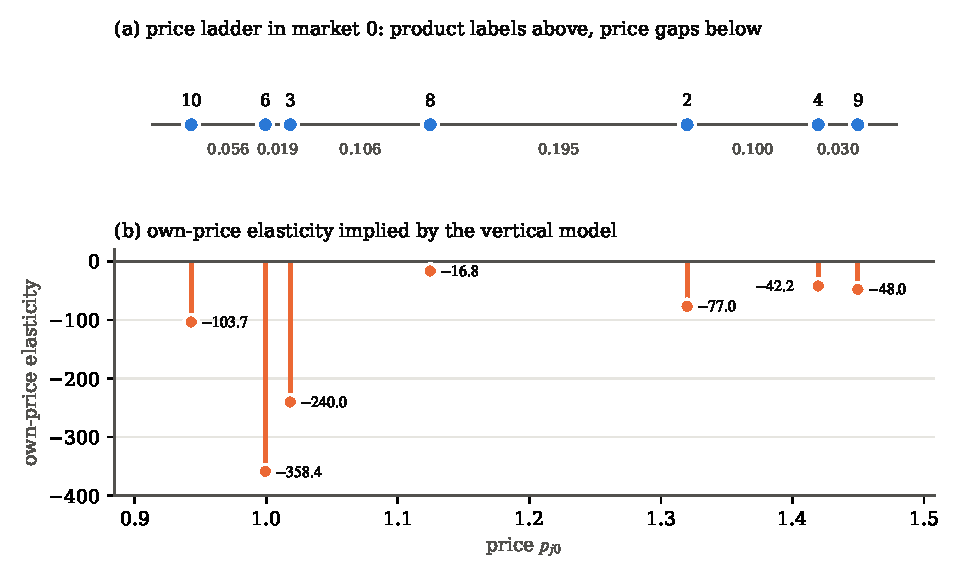
\includegraphics[width=0.9\linewidth]{figures/appC/ladder.pdf}
\caption{The price ladder in market 0. Panel (a) shows the seven prices with the gaps between neighbours. Panel (b)
shows the own-price elasticity $\varepsilon_{jj}$ that the vertical model implies for each product. The products with
the closest neighbours, 6 and 3, have the largest elasticities.}
\label{fig:C-ladder}
\end{figure}

The ladder also governs substitution to the outside good. In the vertical model only the cheapest product loses
customers to the outside good when its price rises. The diversion ratio from product $k$ to the outside good is
\[
  D_{k0} = -\frac{\partial s_0}{\partial p_k}\Big(\frac{\partial s_k}{\partial p_k}\Big)^{-1},
\]
the fraction of the sales that $k$ loses which go to the outside good. For product 10 it is 0.064. Every other product diverts
nothing to the outside good. The logit of \cref{sec:C-logit-est} puts these diversion ratios between 0.86 and 0.91, much
closer to the true model, in which most consumers who leave a product stop buying yogurt (\cref{sec:C-rc-est}).

\casehead{Part (f)}
The vertical model is appropriate when products differ mainly along one quality dimension that all consumers value in
the same direction. Consumers should differ mainly in income or in their marginal utility of money. Then the price
ladder is a quality ladder, and neighbours on it are the natural substitutes. \citet{Bresnahan1987} uses this structure
for the 1955 automobile price war. His consumers have utility $U = vx + Y - P$ from a car of quality $x$ and price $P$,
with $v$ uniform on $[0, V_{\max}]$ with density $d$ (eq.~1, p.~460, and p.~461). Bresnahan writes $\delta$ for
this density. The demand for a car between
neighbours $h$ and $j$ is linear in prices,
\[
  q_i = d\Big[\frac{P_j - P_i}{x_j - x_i} - \frac{P_i - P_h}{x_i - x_h}\Big]
\]
(eq.~5, p.~462). He notes that the quality difference $x_i - x_h$ measures how close two products are as substitutes,
and that they become perfect substitutes as $x_i$ approaches $x_h$ (p.~462). The same feature produces the large
elasticities of \cref{tab:C-velast}. Bresnahan also shows that demand in this model is continuous and concave across the
point where a neighbour is priced out, so a price equilibrium always exists (footnote~6, p.~462). Because only neighbours
compete, collusive and Nash pricing imply very different markups, which gives his conduct test its power
(\cref{sec:06-bresnahan}). The fact to explain is that 1955 production was 45 percent above that of the two surrounding
years, while quality-adjusted prices were lower (p.~457). In nonnested Cox tests the collusive solution is sustained in
1954 and 1956, and the competitive (Nash) solution in 1955 (abstract, p.~457).

Our simulated market violates the premises. Tastes vary along four dimensions, the products crowd into a narrow price
range, and the outside good takes more than three quarters of every market. The vertical model can explain why consumers
split across products with similar prices only by placing those products almost on top of one another in quality. It
then reads every small price gap as intense competition. Its elasticities are wrong by one to two orders of magnitude,
its markups are close to zero, and its implied costs absorb the error. The data offer two warning signs even without
knowledge of the truth. Qualities explain almost none of their own variation ($R^2 = 0.015$), and the implied Nash
markups are far below what any plausible cost information would allow. A model with an idiosyncratic shock, such as
the logit of \cref{sec:C-logit-est}, avoids the zero cross elasticities by construction.

\subsection{Computational notes}

The computations take a few seconds in total.
\begin{enumerate}
  \item In each market, sort products by price and form $\bar S_{(k)t}$ as reversed cumulative sums of the sorted
  realized shares.
  \item Compute $y_{jt}$ by \eqref{eq:C-vy} with \texttt{log1p} for $\ln(1 - \bar S)$, and run OLS of $y$ on $x$ with the
  clustered variance \eqref{eq:C-clustervar}.
  \item Compute $g_{(k)t}$ from \cref{cor:C-vfree}, fill the tridiagonal $\Delta_t$, form $\Omega_t$ from the owners and
  solve $(\Omega_t \odot \Delta_t^\top)\,a = s_t$ for the markups $-a$.
  \item Check the derivatives with a complex step, and check that the shares implied by the recovered qualities
  reproduce the data (largest error $1.9\times10^{-14}$).
\end{enumerate}
The inversion takes a few lines of code.
\begin{verbatim}
def vertical_delta(p, s, lam):
    order = np.argsort(p)                       # price ladder
    tail = np.cumsum(s[order][::-1])[::-1]      # bar S_(k)
    steps = np.diff(p[order], prepend=0.0)      # p_(k) - p_(k-1)
    delta = np.empty_like(p)
    delta[order] = np.cumsum(steps * -np.log1p(-tail) / lam)
    return delta
\end{verbatim}

\section{Estimating logit demand and recovering costs}\label{sec:C-logit-est}

The logit model becomes a linear regression once shares are inverted, so all the tools of linear instrumental variables
apply. In this problem we estimate it on the simulated market, study the strength of the usual instruments, recover
marginal costs with correct standard errors, and estimate demand and supply jointly. Since the data come from a random
coefficients model, the logit is misspecified. We close by deriving the bias that omitted taste heterogeneity creates in
the logit price coefficient and by measuring it in the simulated sample. The general theory of logit estimation is in \cref{ch:logit}.

\subsection{Statement}

Use the data and \cref{ass:C-est} of \cref{sec:C-vertical}. Demand is now logit:
\begin{equation}\label{eq:C-logit}
  u_{ijt} = \delta^l_{jt} + \epsilon_{ijt}, \qquad \delta^l_{jt} = x_{jt}\beta^l - \alpha^l p_{jt} + \xi_{jt},
\end{equation}
with $\epsilon_{ijt}$ independent type-I extreme value and $u_{i0t} = \epsilon_{i0t}$. Firms set prices in a
multi-product Bertrand-Nash equilibrium.

\begin{enumerate}[label=(\alph*)]
  \item Estimate $(\beta^l, \alpha^l)$. Give the identification argument, justify the instruments, assess their strength
  and report standard errors.
  \item Compute the elasticity matrix for market 0 and discuss it.
  \item Derive the marginal cost equation under the assumed conduct, compute $mc_{jt}$ and estimate
  $(\gamma_1, \gamma_2)$ with standard errors that account for the estimation of $\alpha^l$.
  \item Explain how to estimate demand and supply jointly, and when joint estimation matters. Carry it out.
  \item The true model has a random coefficient on price. Show why the logit price coefficient is then biased even with
  valid instruments, explain why the bias is toward zero in this design, and measure it.
\end{enumerate}

\subsection{Solution}

\casehead{Part (a)}
With logit demand the inside and outside shares are
\[
  s_{jt} = \frac{e^{\delta^l_{jt}}}{1 + \sum_{k}e^{\delta^l_{kt}}}, \qquad s_{0t} = \frac{1}{1 + \sum_{k}e^{\delta^l_{kt}}} .
\]
Dividing the first by the second gives $\frac{s_{jt}}{s_{0t}} = e^{\delta^l_{jt}}$, and taking logs gives the inversion of
\citet[eq.~14, p.~250]{Berry1994},
\begin{equation}\label{eq:C-berry}
  \ln s_{jt} - \ln s_{0t} = x_{jt}\beta^l - \alpha^l p_{jt} + \xi_{jt}.
\end{equation}
The left side is computed from realized shares, with $s_{0t} = 1 - \sum_j s_{jt}$. Equation \eqref{eq:C-berry} is
linear in the parameters, with the unobserved quality $\xi_{jt}$ as its error (\cref{eq:07-logit-inversion}).

Price is endogenous. Firms observe $\xi_{jt}$ when they set prices. A product with higher unobserved quality has a
larger share, and logit markups rise with the firm's share (part (c)), so $\Cov(p_{jt}, \xi_{jt}) > 0$. Let
$\tilde p_{jt}$ be the residual from projecting price on $x_{jt}$. The OLS estimate of the price coefficient then converges
to $-\alpha^l + \frac{\Cov(\tilde p_{jt}, \xi_{jt})}{\Var(\tilde p_{jt})}$, so OLS biases $\alpha^l$ toward zero
(\cref{prop:07-ols-bias}). We need excluded instruments that move price and are uncorrelated with $\xi_{jt}$.

We use seven excluded instruments.
\begin{enumerate}
  \item The price of milk $w_{jt}$. It shifts marginal cost and therefore price, it is excluded from utility, and it is
  independent of $\xi_{jt}$ by \cref{ass:C-est}(iii).
  \item Characteristics of the other products in the market. For each characteristic $k$ of product $j$ owned by firm $f$,
  \citet[eq.~5.8, p.~861]{BerryLevinsohnPakes1995} use the sums $\sum_{r \ne j, r \in \mathcal{J}_f}x_{rk}$ and
  $\sum_{r \notin \mathcal{J}_f}x_{rk}$. We form these sums for sugar content and the organic indicator. Because one
  characteristic is the constant, the numbers of the firm's other products and of rival products, $n^{own}_{jt}$ and
  $n^{riv}_{jt}$, are instruments too. This gives six instruments.
\end{enumerate}
\citet[p.~249]{Berry1994} explains why the second group is valid. Rival characteristics are excluded from $u_{ijt}$, and
they are correlated with prices through the markups in the first-order conditions. Their validity requires that
characteristics and the set of products offered in each market be independent of $\xi_{jt}$, which we add to
\cref{ass:C-est}. In this design characteristics are fixed by product, so the six instruments vary only through
which products a market offers and who owns them. The number of the firm's other products runs from 0 to 3 (mean 1.37),
and the number of rival products from 1 to 8 (mean 4.55).

The parameters $\theta^l = (\beta^l, \alpha^l)$ are identified by the moment conditions
\begin{equation}\label{eq:C-logit-moments}
  \E\big[z_{jt}^\top\xi_{jt}\big] = 0, \qquad z_{jt} = \big(x_{jt}, w_{jt}, \text{six competition instruments}\big),
\end{equation}
together with the rank condition that $\E[z_{jt}^\top(x_{jt}, p_{jt})]$ has full column rank four. Economically,
variation in price that comes from costs and from competition, and is unrelated to unobserved quality, traces out how
shares respond to price. We estimate by \emph{two-stage least squares} (2SLS). With $Y$ the stacked left side of
\eqref{eq:C-berry}, $X = (x, p)$ and $Z$ the instrument matrix, the 2SLS coefficient vector is
\[
  \hat b^l = (\hat X^\top\hat X)^{-1}\hat X^\top Y, \qquad \hat X = Z(Z^\top Z)^{-1}Z^\top X .
\]
Since price enters \eqref{eq:C-berry} with coefficient $-\alpha^l$, $\hat b^l$ estimates $(\beta^l, -\alpha^l)$. Its first
three entries give $\hat\beta^l$, and $\hat\alpha^l$ is minus its price entry. The clustered variance of $\hat b^l$ is
\eqref{eq:C-clustervar} with $X_t$ replaced by $\hat X_t$. The residuals in the middle factor are the 2SLS residuals
$\hat e_t = Y_t - X_t\hat b^l$, computed with the actual regressors (\cref{app:econometrics}).

\Cref{tab:C-firststage} reports the first stage. Instrument strength comes almost entirely from the milk price,
whose coefficient is 0.497 with standard error 0.026, close to the true cost coefficient of 0.5. The cluster-robust Wald
statistic for the seven excluded instruments, divided by seven, is 92.5. With one endogenous regressor this is the
cluster-robust first-stage $F$ statistic of \citet{KleibergenPaap2006}. The homoskedastic $F$ is 74.1 and the partial $R^2$ is
0.446. The milk price alone gives $F = 591.4$. The six competition instruments are jointly weak, with $F = 2.32$ and
$p = 0.039$ given the milk price.

\begin{table}[htbp]
\centering
\caption{First stage: OLS of $p_{jt}$ on the exogenous variables}
\label{tab:C-firststage}
\small
\begin{tabular}{@{}lcc@{}}
\toprule
 & Coefficient & Standard error \\
\midrule
Constant & 0.5778 & (0.0188) \\
Sugar content & 0.2575 & (0.0113) \\
Organic & 0.3138 & (0.0064) \\
Price of milk $w_{jt}$ & 0.4972 & (0.0256) \\
Sugar, firm's other products & 0.0023 & (0.0106) \\
Sugar, rival products & $-0.0042$ & (0.0077) \\
Organic, firm's other products & $-0.0015$ & (0.0068) \\
Organic, rival products & $-0.0009$ & (0.0040) \\
Number of firm's other products & 0.0038 & (0.0116) \\
Number of rival products & 0.0020 & (0.0084) \\
\midrule
$R^2$ & 0.923 & \\
$F$, seven excluded instruments (cluster-robust) & 92.5 & \\
$F$, seven excluded instruments (homoskedastic) & 74.1 & \\
$F$, six competition instruments (cluster-robust) & 2.32 & \\
$F$, milk price only (cluster-robust) & 591.4 & \\
\bottomrule
\end{tabular}

\vspace{3pt}
\begin{minipage}{0.97\textwidth}
\footnotesize Notes: 654 observations. Standard errors clustered by market. The milk-price-only
statistic comes from the regression of price on $(x_{jt}, w_{jt})$.
Computed with \texttt{figures/appC/src/appC\_vertical\_logit.py}.
\end{minipage}
\end{table}

The competition instruments are weak for two reasons. First, logit markups barely respond to competition in this
market. The markup of firm $f$ is $\frac{1}{\alpha^l(1 - S_{ft})}$ (part (c)), and the largest combined share of a
firm is only 0.112, so the implied markups run from 0.379 to 0.426. Changes in the set of competitors cannot move prices
much. Second, the instruments are nearly collinear. Sugar content varies only from 0.64 to 1.35, so each sum of sugar
is close to a multiple of the corresponding count. The correlations are 0.978 for the firm's own products and 0.988 for
rivals. The variance inflation factors of the two sugar sums and the two counts are 40.1, 57.8, 36.1 and 52.2. A
variance inflation factor is $\frac{1}{1 - R_k^2}$, the factor by which collinearity with the other regressors inflates
the variance of coefficient $k$.
\citet[p.~861]{BerryLevinsohnPakes1995} report the same problem, finding the matrix of these linear terms ``nearly not
of full rank.''

\Cref{tab:C-logit-demand} reports the estimates. As expected, OLS gives a smaller price coefficient, 2.330, than 2SLS,
2.641. Hansen's test of the six overidentifying restrictions \citep{Hansen1982} uses the two-step GMM estimator with a
market-clustered weighting matrix. It does not reject, with $J = 8.82$ and $p = 0.18$. The two-step GMM estimate of the
price coefficient is 2.872. With the milk price as the only excluded instrument, 2SLS gives 2.677 (0.415), so the
competition instruments change little.

\begin{table}[htbp]
\centering
\caption{Logit demand estimates}
\label{tab:C-logit-demand}
\small
\begin{tabular}{@{}lcccc@{}}
\toprule
 & OLS & 2SLS & \makecell{2SLS,\\ milk price only} & True \\
\midrule
Constant & $-1.443$ & $-1.184$ & $-1.154$ & $-1.00$ \\
 & (0.226) & (0.329) & (0.334) & \\
Sugar content & 0.119 & 0.190 & 0.198 & 0.20 \\
 & (0.122) & (0.158) & (0.156) & \\
Organic & 0.051 & 0.153 & 0.165 & 0.15 \\
 & (0.097) & (0.141) & (0.142) & \\
Price coefficient $\alpha^l$ & 2.330 & 2.641 & 2.677 & 3.00 \\
 & (0.252) & (0.412) & (0.415) & \\
\midrule
First-stage $F$ (cluster-robust) & & 92.5 & 591.4 & \\
Hansen $J$ ($p$-value) & & 8.82 (0.18) & & \\
$R^2$ & 0.396 & 0.395 & 0.395 & \\
Observations & 654 & 654 & 654 & \\
\bottomrule
\end{tabular}

\vspace{3pt}
\begin{minipage}{0.97\textwidth}
\footnotesize Notes: Dependent variable $\ln s_{jt} - \ln s_{0t}$. Standard errors clustered by
market in parentheses. The table reports $\alpha^l$, minus the coefficient on price. The true values are the mean
parameters of the random coefficients model of \cref{sec:C-simulate}.
Computed with \texttt{figures/appC/src/appC\_vertical\_logit.py}.
\end{minipage}
\end{table}

Consistency of 2SLS here rests on one more condition. Characteristics and milk prices are fixed by product, so the
identifying variation in $w_{jt}$ comes from its ten values across products. If $\xi_{jt}$ contained a persistent
product component, it could correlate with the product-level instruments. An $F$ test of product dummies on the 2SLS
residuals, beyond the product-level regressors, gives $F(6, 644) = 1.18$ with $p = 0.32$. With only ten products the test
has little power, so it cannot rule such a component out. In this design the unobservables are drawn independently
across markets, so the condition holds by construction.

The 2SLS price coefficient, 2.641, lies below the true mean of 3, but only 0.87 standard errors below. The
characteristic coefficients are close to the truth and imprecise, because sugar and organic status take only ten distinct
combinations. Part (e) splits the shortfall in $\hat\alpha^l$. Most of it, 0.284 of 0.359, is an estimate of the
misspecification bias of the logit. The rest reflects sampling and simulation error, since the random coefficients model
gives 2.926 on the same sample.

\casehead{Part (b)}
The logit share derivatives of \cref{sec:C-logit-bertrand}, part (a), hold with $\alpha^l$ in place of $\alpha$
(\cref{prop:07-logit-derivs}). They give the elasticities \eqref{eq:C-logit-elast} together with the outside-good row,
\begin{equation}\label{eq:C-lelast}
  \varepsilon_{jj} = -\alpha^l p_j(1 - s_j), \qquad \varepsilon_{jk} = \alpha^l p_ks_k \quad (k \ne j), \qquad
  \varepsilon_{0k} = \alpha^l p_ks_k .
\end{equation}
\Cref{tab:C-lelast} evaluates them at $\hat\alpha^l = 2.641$ and the observed prices and realized shares of market 0.

\begin{table}[htbp]
\centering
\caption{Logit model: price elasticities in market 0}
\label{tab:C-lelast}
\small
\begin{tabular}{@{}lrrrrrrr@{}}
\toprule
 & \multicolumn{7}{c}{Price of product} \\
\cmidrule(lr){2-8}
Share of & 2 & 3 & 4 & 6 & 8 & 9 & 10 \\
\midrule
Product 2 & $-3.47$ & 0.07 & 0.05 & 0.05 & 0.17 & 0.02 & 0.05 \\
Product 3 & 0.02 & $-2.62$ & 0.05 & 0.05 & 0.17 & 0.02 & 0.05 \\
Product 4 & 0.02 & 0.07 & $-3.70$ & 0.05 & 0.17 & 0.02 & 0.05 \\
Product 6 & 0.02 & 0.07 & 0.05 & $-2.59$ & 0.17 & 0.02 & 0.05 \\
Product 8 & 0.02 & 0.07 & 0.05 & 0.05 & $-2.80$ & 0.02 & 0.05 \\
Product 9 & 0.02 & 0.07 & 0.05 & 0.05 & 0.17 & $-3.81$ & 0.05 \\
Product 10 & 0.02 & 0.07 & 0.05 & 0.05 & 0.17 & 0.02 & $-2.44$ \\
Outside good & 0.02 & 0.07 & 0.05 & 0.05 & 0.17 & 0.02 & 0.05 \\
\bottomrule
\end{tabular}

\vspace{3pt}
\begin{minipage}{0.97\textwidth}
\footnotesize Notes: Entry $(j, k)$ is $\varepsilon_{jk}$ from \eqref{eq:C-lelast} with
$\hat\alpha^l = 2.641$ (2SLS), evaluated at observed prices and realized shares. Computed with \texttt{figures/appC/src/appC\_vertical\_logit.py}.
\end{minipage}
\end{table}

The own elasticities run from $-2.44$ to $-3.81$, so every product faces elastic demand. Across all 654 observations
they lie between $-2.21$ and $-4.24$, with mean $-3.06$. They are close to the true values, $-2.57$ to $-3.85$ in market
0, but slightly smaller in magnitude, because $\hat\alpha^l$ is below 3. Since shares are small,
$\varepsilon_{jj} \approx -\alpha^l p_j$, so the model makes the most expensive products the most elastic by
construction. Products 9 and 4, the two most expensive, have the largest own elasticities.

Every off-diagonal entry in a column is the same, and it equals the outside-good entry. This is the independence of
irrelevant alternatives. A rise in $p_k$ raises the shares of all other products and of the outside good in the same
proportion, whatever their characteristics. Diversion from product $k$ to the outside good is
$D_{k0} = \frac{\alpha^l s_0s_k}{\alpha^l s_k(1 - s_k)} = \frac{s_0}{1 - s_k}$, between 0.86 and 0.91 in market 0. In the
true model a price rise for an organic product diverts more customers to the other organic products and to expensive
products (\cref{sec:C-rc-est}). The logit cannot produce this pattern.

\casehead{Part (c)}
With logit demand the first-order conditions \eqref{eq:C-vsupply-nash} reduce to the common-markup rule of
\cref{prop:C-common-markup}, derived in \cref{sec:C-logit-bertrand}, part (e) (see also \cref{prop:07-logit-multi}).
Every product of firm $f$ in market $t$ carries the markup $m_{ft} = \frac{1}{\alpha^l(1 - S_{ft})}$, where
$S_{ft} = \sum_{k \in \mathcal{J}_{ft}}s_{kt}$ is the firm's combined share. The marginal cost equation is
\begin{equation}\label{eq:C-lsupply}
  mc_{jt} = p_{jt} - \frac{1}{\alpha^l(1 - S_{ft})} = x_{jt}\gamma_1 + \gamma_2 w_{jt} + \omega_{jt} .
\end{equation}
This is \eqref{eq:C-vsupply-nash} with the logit Jacobian. The script confirms that the closed form and the matrix formula
agree to $2.2\times10^{-16}$. We compute $mc_{jt}$ with $\hat\alpha^l = 2.641$ and the realized shares. The implied
markups run from 0.379 to 0.426 with mean 0.396, against a true mean of 0.386. Their correlation with the true markups
is 0.55, against 0.27 for the vertical Nash markups. No implied marginal cost is negative. Identification of
$(\gamma_1, \gamma_2)$ follows as in \cref{sec:C-vertical}, from $\E[\omega_{jt} \mid x_{jt}, w_{jt}] = 0$ and full rank.
We estimate it by OLS of $mc_{jt}$ on $(x_{jt}, w_{jt})$.

The dependent variable now contains the estimate $\hat\alpha^l$. Clustered OLS standard errors treat $mc_{jt}$ as data
and so ignore this uncertainty. We correct them in two ways.

The first is a \emph{market bootstrap}. Each of 5,000 replications draws 100 markets with replacement, re-estimates
$(\beta^l, \alpha^l)$ by 2SLS, recomputes every implied marginal cost with the new $\alpha^l$, and re-runs the supply
regression. The bootstrap standard error is the standard deviation of the replicated estimates. Resampling whole markets
preserves dependence within markets and is valid because markets are independent. With 5,000 replications the Monte
Carlo error of each bootstrap standard error of the cost coefficients is below 0.0011.

The second treats the two steps as one GMM estimator with stacked moments \citep{Newey1984, MurphyTopel1985}. Write
$k_{jt} = \frac{1}{1 - S_{ft}}$, so that $mc_{jt}(\alpha) = p_{jt} - \frac{k_{jt}}{\alpha}$, and let $W$ be the regressor
matrix of \eqref{eq:C-supplydecomp}, with rows $W_{jt} = (x_{jt}, w_{jt})$. The supply estimate solves
$\sum_{t}\sum_j W_{jt}^\top\big(p_{jt} - \frac{k_{jt}}{\hat\alpha^l} - W_{jt}\hat\gamma\big) = 0$. A first-order expansion
around the probability limits gives
\begin{equation}\label{eq:C-stacked}
  \begin{aligned}
  \hat\gamma - \gamma &\approx (W^\top W)^{-1}\Big[\sum_{t}\sum_j W_{jt}^\top\omega_{jt}
  + \frac{W^\top k}{(\alpha^l)^2}\big(\hat\alpha^l - \alpha^l\big)\Big], \\
  \hat\alpha^l - \alpha^l &\approx -\iota_p^\top(\hat X^\top\hat X)^{-1}\sum_{t}\sum_j\hat X_{jt}^\top\xi_{jt},
  \end{aligned}
\end{equation}
where $\iota_p$ selects the price coefficient. Each observation thus contributes an influence term to $\hat\gamma$.
Summing these terms within markets and taking the clustered outer product gives a sandwich variance that includes the
estimation error in $\alpha^l$. The coefficient $(W^\top W)^{-1}\frac{W^\top k}{(\alpha^l)^2}$ measures how the cost estimates
move with $\alpha^l$. For the constant it is 0.148, close to the mean markup divided by $\alpha^l$. With
$\text{s.e.}(\hat\alpha^l) = 0.412$, this alone gives a standard error of about $0.148 \times 0.412 = 0.061$ for the
intercept. \Cref{tab:C-lsupply} reports the estimates.

\begin{table}[htbp]
\centering
\caption{Logit model, supply side: OLS of the implied marginal cost on $(x_{jt}, w_{jt})$}
\label{tab:C-lsupply}
\small
\setlength{\tabcolsep}{5pt}
\begin{tabular}{@{}lcccccc@{}}
\toprule
 & Estimate & \makecell{Clustered\\ s.e.} & \makecell{Stacked\\ s.e.} & \makecell{Bootstrap\\ s.e.}
 & \makecell{Bootstrap\\ 95\% interval} & True \\
\midrule
Constant & 0.160 & 0.016 & 0.065 & 0.072 & $[-0.022, 0.257]$ & 0.20 \\
Sugar content & 0.258 & 0.010 & 0.010 & 0.010 & $[0.239, 0.278]$ & 0.25 \\
Organic & 0.315 & 0.005 & 0.006 & 0.006 & $[0.304, 0.327]$ & 0.30 \\
Price of milk & 0.532 & 0.023 & 0.023 & 0.023 & $[0.487, 0.576]$ & 0.50 \\
\bottomrule
\end{tabular}

\vspace{3pt}
\begin{minipage}{0.97\textwidth}
\footnotesize Notes: The implied marginal cost is \eqref{eq:C-lsupply} with $\hat\alpha^l = 2.641$, and
$R^2 = 0.923$. The clustered standard errors treat $mc_{jt}$ as data. The stacked standard errors use the influence
functions in \eqref{eq:C-stacked}, clustered by market. The bootstrap resamples markets 5,000 times and re-estimates
$\alpha^l$ in each replication. The interval is the percentile interval.
Computed with \texttt{figures/appC/src/appC\_vertical\_logit.py}.
\end{minipage}
\end{table}

The estimates are close to the true values. Uncertainty about $\alpha^l$ moves all markups together, since each is near
$\frac{1}{\alpha^l}$ when shares are small. It therefore loads almost entirely on the intercept, whose standard error rises
from 0.016 to 0.065 (stacked) or 0.072 (bootstrap), while the slope standard errors barely change. The two corrections
agree closely. The decomposition \eqref{eq:C-supplydecomp} locates the remaining errors. The logit markup error loads
$-0.040$ on the constant, $0.011$ on sugar, $0.011$ on organic and $0.030$ on the milk price. True markups are higher for
organic products (0.392 against 0.383), because their buyers are less price sensitive. Logit markups are slightly lower
for them (0.392 against 0.397), because organic producers have smaller combined shares. The logit therefore understates
the organic markup premium ($-0.005$ against $+0.008$ in the truth), so it overstates the organic cost premium. The
bootstrap interval for the organic coefficient just excludes 0.30.
Compared with the vertical model under Nash pricing (\cref{tab:C-vsupply}), the logit recovers costs far more accurately
because its markups are close to the true ones.

\casehead{Part (d)}
Joint estimation stacks the demand and supply moments and estimates
$\theta = (\beta^l, \alpha^l, \gamma_1, \gamma_2)$ by GMM. For a candidate $\theta$, the residuals are
\begin{equation}\label{eq:C-joint-resid}
  \xi_{jt}(\theta) = \ln s_{jt} - \ln s_{0t} - x_{jt}\beta^l + \alpha^l p_{jt}, \qquad
  \omega_{jt}(\theta) = p_{jt} - \frac{1}{\alpha^l(1 - S_{ft})} - x_{jt}\gamma_1 - \gamma_2 w_{jt}.
\end{equation}
With demand instruments $z^d_{jt}$ and supply instruments $z^s_{jt}$, the sample moments and the estimator are
\begin{equation}\label{eq:C-joint}
  \bar g(\theta) = \frac{1}{N}\sum_{t}\sum_j\begin{pmatrix} z^{d\top}_{jt}\,\xi_{jt}(\theta) \\
  z^{s\top}_{jt}\,\omega_{jt}(\theta)\end{pmatrix}, \qquad
  \hat\theta = \argmin_\theta \bar g(\theta)^\top\,\mathcal W\,\bar g(\theta).
\end{equation}
The first step uses the block-diagonal weight $\mathcal W_1 = \diag\big((\frac{1}{N}Z^{d\top}Z^d)^{-1},
(\frac{1}{N}Z^{s\top}Z^s)^{-1}\big)$. The second step uses the inverse of the market-clustered covariance of the moments
at the first-step estimate, $\mathcal W_2 = \hat S^{-1}$, which is efficient. Given $\alpha^l$, both residuals are linear in
$(\beta^l, \gamma_1, \gamma_2)$, so we concentrate these out by weighted least squares and search over $\alpha^l$ alone.
The GMM sandwich then gives standard errors that account for the estimation of $\alpha^l$ in the markups
(\cref{sec:08-supply-joint}).

\begin{proposition}[A just-identified supply block adds nothing]\label{prop:C-redundant}
Let $z^s_{jt} = (x_{jt}, w_{jt})$, so that the supply block has as many moments as cost parameters. Then the joint GMM
estimate of $(\beta^l, \alpha^l)$ with weight $\mathcal W$ equals the GMM estimate from the demand moments alone with weight
$\mathcal W_{dd} - \mathcal W_{ds}\mathcal W_{ss}^{-1}\mathcal W_{sd}$. With the block-diagonal $\mathcal W_1$ this is 2SLS. With
the efficient $\mathcal W_2 = \hat S^{-1}$ it is two-step efficient GMM on the demand moments with weight $\hat S_{dd}^{-1}$.
\end{proposition}

\begin{proof}
Partition $\bar g = (\bar g_d, \bar g_s)$. For fixed $(\beta^l, \alpha^l)$, $\bar g_s = b_s(\alpha^l) - \frac{1}{N}W^\top
W\gamma$, and $\frac{1}{N}W^\top W$ is square and invertible. Choosing $\gamma$ is therefore the same as choosing the value
$v$ of $\bar g_s$ freely. Minimizing the quadratic form over $v$,
\[
  \min_v\begin{pmatrix}\bar g_d \\ v\end{pmatrix}^\top
  \begin{pmatrix}\mathcal W_{dd} & \mathcal W_{ds} \\ \mathcal W_{sd} & \mathcal W_{ss}\end{pmatrix}
  \begin{pmatrix}\bar g_d \\ v\end{pmatrix}
  = \bar g_d^\top\big(\mathcal W_{dd} - \mathcal W_{ds}\mathcal W_{ss}^{-1}\mathcal W_{sd}\big)\bar g_d ,
\]
attained at $v = -\mathcal W_{ss}^{-1}\mathcal W_{sd}\bar g_d$. The concentrated objective involves only the demand
moments. For block-diagonal $\mathcal W$ the bracket is $\mathcal W_{dd}$. For $\mathcal W = \hat S^{-1}$, the formula for the
inverse of a partitioned matrix gives $\mathcal W_{dd} - \mathcal W_{ds}\mathcal W_{ss}^{-1}\mathcal W_{sd} = \hat S_{dd}^{-1}$.
\end{proof}

This is a special case of a general separability result for GMM \citep{AhnSchmidt1995}. The supply side carries
information about demand only when it has more moments than cost parameters. Under \cref{ass:C-est}(iii), $\omega_{jt}$ is
also independent of the characteristics of other products, so the six competition instruments are valid supply
instruments. \citet[p.~255]{Berry1994} proposes the characteristics of other firms as cost-side instruments for the same
reason. \citet[pp.~861--862]{BerryLevinsohnPakes1995} interact their cost error with the three terms of their eq.~(5.8)
for each of six cost characteristics. The three terms are the characteristic itself, its sum over the firm's other
products and its sum over rival products. They add miles per dollar, a demand variable excluded from cost, for nineteen cost-side
instruments in all.

With these instruments the supply equation identifies $\alpha^l$ on its own. Rewrite \eqref{eq:C-lsupply} as
\begin{equation}\label{eq:C-supply-only}
  p_{jt} = x_{jt}\gamma_1 + \gamma_2 w_{jt} + \frac{1}{\alpha^l}\,k_{jt} + \omega_{jt}, \qquad k_{jt} = \frac{1}{1 - S_{ft}} ,
\end{equation}
a linear regression in which $\frac{1}{\alpha^l}$ is the coefficient on $k_{jt}$. This is the multi-product version of the
logit supply equation of \citet[eq.~31, p.~255]{Berry1994}, whose parameters are $\gamma$ and $\frac{1}{\alpha}$. The firm
share is endogenous, because a high $\omega_{jt}$ raises the price and lowers the share. The competition instruments predict
$k_{jt}$ well, with a cluster-robust first-stage $F$ of 51.6. The number and type of a firm's other products move its
combined share directly. 2SLS of \eqref{eq:C-supply-only} gives $\frac{1}{\hat\alpha^l} = 0.351$ (0.132), so
$\hat\alpha^l = 2.85$ with a delta-method standard error of 1.07. The estimate is close to the demand-side values, but it
is imprecise because $k_{jt}$ varies only from 1.002 to 1.126. The markups move too little across markets to measure their
slope well. \Cref{tab:C-joint} shows what the joint estimator does with this extra information.

\begin{table}[htbp]
\centering
\caption{Sequential and joint estimation of logit demand and supply}
\label{tab:C-joint}
\small
\begin{tabular}{@{}lcccc@{}}
\toprule
 & Sequential & \makecell{Joint GMM,\\ $z^s = (x, w)$} & \makecell{Joint GMM, $z^s$ adds\\ six instruments}
 & True \\
\midrule
\multicolumn{5}{l}{\textit{Demand}} \\
Constant & $-1.184$ (0.329) & $-1.035$ (0.311) & $-1.101$ (0.291) & $-1.00$ \\
Sugar content & 0.190 (0.158) & 0.291 (0.152) & 0.267 (0.144) & 0.20 \\
Organic & 0.153 (0.141) & 0.211 (0.134) & 0.178 (0.123) & 0.15 \\
Price coefficient $\alpha^l$ & 2.641 (0.412) & 2.872 (0.394) & 2.785 (0.367) & 3.00 \\
\multicolumn{5}{l}{\textit{Marginal cost}} \\
Constant & 0.160 (0.072) & 0.191 (0.053) & 0.181 (0.053) & 0.20 \\
Sugar content & 0.258 (0.010) & 0.261 (0.010) & 0.260 (0.009) & 0.25 \\
Organic & 0.315 (0.006) & 0.315 (0.005) & 0.314 (0.005) & 0.30 \\
Price of milk & 0.532 (0.023) & 0.529 (0.022) & 0.527 (0.021) & 0.50 \\
\midrule
Moments & & 14 & 20 & \\
Hansen $J$ (d.f., $p$) & & 8.82 (6, 0.18) & 12.85 (12, 0.38) & \\
\bottomrule
\end{tabular}

\vspace{3pt}
\begin{minipage}{0.97\textwidth}
\footnotesize Notes: The sequential column is 2SLS for demand (clustered standard errors) and OLS
for supply (bootstrap standard errors). The joint columns are two-step efficient GMM estimates of \eqref{eq:C-joint} with
$z^d$ as in part (a), weights clustered by market, and GMM sandwich standard errors without a small-sample factor. With
$z^s = (x, w)$ the first step reproduces the sequential point estimates (\cref{prop:C-redundant}). With the six added
supply instruments the first step gives $\hat\alpha^l = 2.642$, which differs slightly from the sequential 2.641.
Computed with \texttt{figures/appC/src/appC\_vertical\_logit.py}.
\end{minipage}
\end{table}

The numbers confirm \cref{prop:C-redundant}. With $z^s = (x, w)$, the first-step joint estimate of $\alpha^l$ is 2.641, the
2SLS value. The second-step estimate is 2.872, exactly the two-step GMM estimate from the demand moments alone, and the
$J$ statistic is the same 8.82. The cost coefficients do change, because the efficient weight lets demand residuals inform
the supply block. Adding the six competition instruments to the supply side changes even the first step, which gives
2.642. The cost parameters can no longer set every supply moment to zero, and the remaining supply moments depend on
$\alpha^l$ through the markups. The second step gives $\hat\alpha^l = 2.785$ with standard error 0.367, against 0.394
without the added instruments. The estimate is close to the demand-side estimates and to the supply-only value of
2.85. The gain in precision is modest, for the reason that made these instruments weak in the first stage. With combined shares
of at most 0.112, the markups barely change with competition. The overidentifying restrictions are not rejected
($J = 12.85$ with 12 degrees of freedom, $p = 0.38$).

Joint estimation matters in four situations. The first is when demand moments identify the demand parameters poorly,
because instruments are weak or because there are nonlinear parameters such as the random coefficients of
\cref{sec:C-rc-est}. Extra supply moments then add information. The second is when $\xi_{jt}$ and $\omega_{jt}$ are
correlated and the supply block is overidentified, since the efficient weight then links the blocks. The third is when
conduct itself is a parameter, because only the supply side identifies it. The fourth is when correct standard errors for
the cost parameters are needed and no bootstrap is run. Joint estimation also has a cost. If the conduct assumption is
wrong, the supply moments contaminate the demand estimates, which sequential estimation protects against.

\casehead{Part (e)}
The true model of \cref{sec:C-simulate} has random coefficients, $u_{ijt} = \delta_{jt} + \tilde x_{jt}\Sigma\nu_i +
\epsilon_{ijt}$ with $\tilde x_{jt} = (x_{jt}, p_{jt})$, $\nu_i \sim N(0, I_4)$ and $\delta_{jt} = x_{jt}\beta - \alpha
p_{jt} + \xi_{jt}$. Let $\delta_{jt}$ be the mean utility that rationalizes the observed shares in this model, recovered
by the contraction of \cref{thm:08-contraction}, which \cref{prop:C-blp-contraction} of the next problem verifies for
this market. Define the \emph{gap term}
\begin{equation}\label{eq:C-gap}
  r_{jt} = \ln\frac{s_{jt}}{s_{0t}} - \delta_{jt} .
\end{equation}
The logit regression \eqref{eq:C-berry} then has the dependent variable $x_{jt}\beta - \alpha p_{jt} + \xi_{jt} +
r_{jt}$, so its error is $\xi_{jt} + r_{jt}$.

\begin{proposition}[Decomposition of the logit estimate]\label{prop:C-logit-bias}
Use the regressors $(x_{jt}, p_{jt})$ and the instruments $z_{jt}$ throughout. Let $\hat b^{RC}$ be the 2SLS coefficient
vector with dependent variable $\delta_{jt}$, and let $\hat b^l$ be the one with dependent variable $\ln\frac{s_{jt}}{s_{0t}}$.
Write $\hat\alpha^{RC}$ and $\hat\alpha^l$ for minus their price entries. Let $\hat b_r$ be the one with dependent
variable $r_{jt}$, with price coefficient $\hat b_{r,p}$. Then
\begin{equation}\label{eq:C-decomp}
  \hat b^l = \hat b^{RC} + \hat b_r, \qquad \hat\alpha^l = \hat\alpha^{RC} - \hat b_{r,p}.
\end{equation}
Suppose the random coefficients model is correct and $z_{jt}$ is valid for it. Then $\plim\hat\alpha^l = \alpha - b_{r,p}$,
where $b_{r,p}$ is the price coefficient of the population 2SLS projection of $r_{jt}$ on $(x_{jt}, p_{jt})$ with
instruments $z_{jt}$. The logit estimate is biased toward zero whenever $b_{r,p} > 0$.
\end{proposition}

\begin{proof}
The 2SLS estimator is linear in the dependent variable, $\hat b(Y) = (X^\top P_ZX)^{-1}X^\top P_ZY$ with
$P_Z = Z(Z^\top Z)^{-1}Z^\top$. Since $\ln\frac{s_{jt}}{s_{0t}} = \delta_{jt} + r_{jt}$ observation by observation,
$\hat b^l = \hat b(\delta) + \hat b(r) = \hat b^{RC} + \hat b_r$. The price coefficient is $-\alpha$ in both models, so
the price entries give $-\hat\alpha^l = -\hat\alpha^{RC} + \hat b_{r,p}$, which is the second equation. Under the
stated conditions $\plim\hat\alpha^{RC} = \alpha$, and $\hat b_{r,p}$ converges to its population counterpart.
\end{proof}

The instruments do not remove this bias. The gap term depends on prices, and prices depend on the milk price and on the
competition instruments, so $\E[z_{jt}^\top r_{jt}] \ne 0$ in general. The question is the sign of $b_{r,p}$. No general
result fixes it, because it depends on the model, the design and the instruments. The next result shows how $r_{jt}$
varies across the products of one market when tastes are only slightly dispersed.

\begin{proposition}[The gap term for small taste dispersion]\label{prop:C-gap-approx}
Let $\Sigma$ be diagonal and $\nu_i \sim N(0, I_4)$. As $\lVert\Sigma\rVert \to 0$,
\begin{equation}\label{eq:C-gap-approx}
  r_{jt} = \frac{1}{2}\,\tilde x_{jt}\Sigma^2\tilde x_{jt}^\top - \tilde x_{jt}\Sigma^2\bar x_t^\top + O(\lVert\Sigma\rVert^3),
  \qquad \bar x_t = \sum_{k}s_{kt}\tilde x_{kt},
\end{equation}
where the sum runs over inside products. In particular, the price component of $r_{jt}$ is
$\Sigma_{pp}^2\big(\frac{1}{2}p_{jt}^2 - p_{jt}\bar p_t\big)$, with $\Sigma_{pp}$ the price entry of $\Sigma$ and
$\bar p_t = \sum_k s_{kt}p_{kt}$. All products of market $t$ share $\bar p_t$, so among the products of a market priced
above $\bar p_t$ this component is larger for the more expensive product.
\end{proposition}

\begin{proof}
Fix a market and drop $t$. Let $\mu_{ij} = \tilde x_j\Sigma\nu_i$ for inside goods and $\mu_{i0} = 0$. Write
$s^L_j$ for the logit shares at $\delta$, so that $\ln\frac{s^L_j}{s^L_0} = \delta_j$. The individual choice probability is
the logit probability at utilities $\delta_j + \mu_{ij}$. Since $\frac{\partial\ln s_j}{\partial u_k} = \indic\{j = k\} -
s_k$ and $\frac{\partial^2\ln s_j}{\partial u_k\partial u_l} = -s_k(\indic\{k = l\} - s_l)$, a second-order expansion in
$\mu_i$ gives
\[
  \ln s_{ij} = \ln s^L_j + \mu_{ij} - \bar\mu_i - \frac{1}{2}V_i + O(|\mu_i|^3), \qquad
  \bar\mu_i = \sum_k s^L_k\mu_{ik}, \quad V_i = \sum_k s^L_k\mu_{ik}^2 - \bar\mu_i^2 ,
\]
for every alternative, including $j = 0$ with $\mu_{i0} = 0$. Exponentiating and expanding,
\[
  s_{ij} = s^L_j\Big[1 + (\mu_{ij} - \bar\mu_i) - \frac{1}{2}V_i + \frac{1}{2}(\mu_{ij} - \bar\mu_i)^2\Big] + O(|\mu_i|^3).
\]
Average over $\nu_i$. Because $\E[\mu_{ij}] = 0$ and $\mu_i = O(\lVert\Sigma\rVert)$,
\[
  s_j = s^L_j\Big[1 + \frac{1}{2}\E(\mu_{ij} - \bar\mu_i)^2 - \frac{1}{2}\E V_i\Big] + O(\lVert\Sigma\rVert^3), \qquad
  s_0 = s^L_0\Big[1 + \frac{1}{2}\E\bar\mu_i^2 - \frac{1}{2}\E V_i\Big] + O(\lVert\Sigma\rVert^3).
\]
Take logs, use $\ln(1 + a) = a + O(a^2)$ with $a = O(\lVert\Sigma\rVert^2)$, and subtract:
\[
  \ln\frac{s_j}{s_0} - \delta_j = \frac{1}{2}\E\big[(\mu_{ij} - \bar\mu_i)^2 - \bar\mu_i^2\big] + O(\lVert\Sigma\rVert^3)
  = \frac{1}{2}\E[\mu_{ij}^2] - \E[\mu_{ij}\bar\mu_i] + O(\lVert\Sigma\rVert^3).
\]
With $\nu_i \sim N(0, I_4)$ and $\Sigma$ diagonal, $\E[\mu_{ij}^2] = \tilde x_j\Sigma^2\tilde x_j^\top$ and
$\E[\mu_{ij}\bar\mu_i] = \tilde x_j\Sigma^2\big(\sum_k s^L_k\tilde x_k\big)^\top$. Finally $s^L_k - s_k = O(\lVert\Sigma\rVert^2)$,
and the term it multiplies is $O(\lVert\Sigma\rVert^2)$, so replacing $s^L_k$ by $s_k$ changes $r_j$ by $O(\lVert\Sigma\rVert^4)$.
For fixed $\bar p$, the price component $\Sigma_{pp}^2(\frac{1}{2}p^2 - p\bar p)$ has derivative $\Sigma_{pp}^2(p - \bar p)$ in
the product's own price $p$, which is positive for $p > \bar p$.
\end{proof}

The comparison in \cref{prop:C-gap-approx} holds $\bar p_t$ fixed, as it is across the products of one market. It does not
give the response of $r_{jt}$ to a change in $p_{jt}$, which also moves the shares and hence $\bar p_t$. To leading order
the logit share derivatives give $\frac{\partial\bar p_t}{\partial p_{jt}} = s_{jt}\big[1 - \alpha(p_{jt} - \bar p_t)\big]$,
so the full derivative of the price component is
\begin{equation*}
  \Sigma_{pp}^2\Big[(p_{jt} - \bar p_t)(1 + \alpha p_{jt}s_{jt}) - p_{jt}s_{jt}\Big] .
\end{equation*}
It can be negative for a product with a large share. With one inside good, $p = 1$, $\alpha = 1$ and share
$\frac{3}{4}$, it equals $-\frac{5}{16}\Sigma_{pp}^2$, although $p$ exceeds $\bar p = \frac{3}{4}$. Neither derivative
signs $b_{r,p}$ by itself. The 2SLS projection pools products and markets with different $\bar p_t$, and the instruments
decide which price variation it uses. The sign of the bias is therefore specific to the model, the design and the
instruments.

Our design, with small inside shares, is a favorable case for a positive $b_{r,p}$. The outside share is at least 0.788 in every market, so
$\bar p_t$ lies between 0.064 and 0.224, while every price is at least 0.881. Every observation has
$p_{jt} - \bar p_t \ge 0.707$. At the random coefficients estimate of $\alpha$ reported below, the full derivative is at
least $0.729\,\Sigma_{pp}^2$ at every observation. Both derivatives are therefore positive throughout the sample.

The intuition is sorting. Consumers with a low price sensitivity $\alpha_i = \alpha - \Sigma_{pp}\nu_{i4}$ buy expensive
products more than the average consumer does. Averaging the convex logit probability over this heterogeneity raises the
share of expensive products above what a logit with the same mean utility predicts. The logit can absorb the excess only
in its error term, which is then larger for the more expensive products of a market. By \eqref{eq:C-gap-approx}, the
within-market slope of the price component is $\Sigma_{pp}^2(p_{jt} - \bar p_t)$. With $\Sigma_{pp} = 0.5$, a mean price of
1.18 and a mean $\bar p_t$ of 0.142 across observations, this slope averages 0.259.

We now compute each term of \eqref{eq:C-decomp} in our sample. The script recovers $\delta_{jt}$ in every market by the
contraction with 1,000 fixed draws per market (seed 2030), as in \cref{sec:C-rc-est}. Convergence to a tolerance of $10^{-10}$ takes 11 to 18
iterations. \Cref{fig:C-gap} plots $r_{jt}$ against price. The gap is positive for every observation, from 0.105 to
0.511, so every recovered $\delta_{jt}$ lies below its logit start (\cref{prop:C-delta-lower}). Its correlation with price
is 0.888. In market 0 it rises from 0.125 for the cheapest product to 0.326 for the
most expensive one. The 2SLS estimate of the random coefficients model on the same sample and instruments is
$\hat\alpha^{RC} = 2.926$ (0.413). The 2SLS price coefficient of $r_{jt}$ is $\hat b_{r,p} = 0.284$, and the identity
\eqref{eq:C-decomp}, $2.641 = 2.926 - 0.284$, holds to $9\times10^{-16}$. The approximation \eqref{eq:C-gap-approx},
evaluated at the true $\Sigma$, has correlation 0.93 with the exact $r_{jt}$. Its own 2SLS price coefficient is 0.286, and
its price component alone gives 0.270.

\begin{figure}[htbp]
\centering
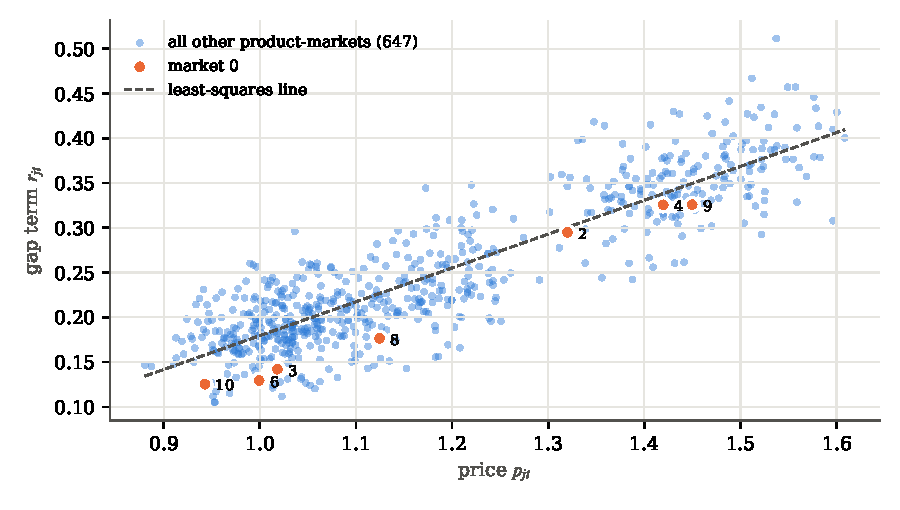
\includegraphics[width=0.85\linewidth]{figures/appC/gap.pdf}
\caption{The gap term $r_{jt} = \ln\frac{s_{jt}}{s_{0t}} - \delta_{jt}$ against price for all 654 observations, with market 0
highlighted and its products labelled. $\delta_{jt}$ is the random coefficients mean utility recovered with the true
$\Sigma$. The correlation with price is 0.888. The dashed simple least-squares line has slope 0.378. The 2SLS price
coefficient, which controls for characteristics, is 0.284.}
\label{fig:C-gap}
\end{figure}

The estimated bias $\hat b_{r,p} = 0.284$ is about 0.7 standard errors of $\hat\alpha^l$, so a single sample cannot
detect it. It comes from one sample of 654 observations, with 1,000 simulation draws per market, so it contains
sampling and simulation error. Its population counterpart $b_{r,p}$ is the probability limit of the bias
(\cref{prop:C-logit-bias}). Unlike sampling error, $b_{r,p}$ does not shrink as the number of markets grows. The
consequences of the bias also propagate. A price coefficient that is too small makes demand look too inelastic,
which inflates the logit markups $\frac{1}{\alpha^l(1 - S_{ft})}$ to a mean of 0.396 against the true 0.386. Better instruments cannot repair it, because the problem lies in the functional form.
The remedy is to model the heterogeneity, which \cref{sec:C-rc-est} does. \Cref{sec:08-worked} reports the same comparison
within the full estimation of the random coefficients model.

\subsection{Computational notes}

\begin{enumerate}
  \item Build the instruments with group sums: within each market and owner, sum each characteristic and subtract the
  product's own value for the firm's other products. The market sum minus the firm sum gives the rival products.
  \item Compute 2SLS through the projected regressors $\hat X$. Code the clustered sandwich by hand and check it against
  a packaged routine. Here the coefficients and standard errors agree to within $2\times10^{-12}$.
  \item For Hansen's $J$, run 2SLS, form $\hat S = \frac{1}{N}\sum_t(Z_t^\top\hat e_t)(Z_t^\top\hat e_t)^\top$ from its
  residuals, re-estimate with weight $\hat S^{-1}$, and compute $J = N\bar g^\top\hat S^{-1}\bar g$ at the second-step
  estimate.
  \item For the bootstrap, note that $mc_{jt}(\alpha) = p_{jt} - \frac{k_{jt}}{\alpha}$ with $k_{jt}$ fixed by the data,
  so each replication needs only one 2SLS fit and one OLS fit.
  \item For joint GMM, concentrate out the linear parameters for each $\alpha^l$ by weighted least squares, minimize the
  concentrated objective over a grid and refine with a bounded scalar search.
  \item For the gap term, run the contraction from the logit start $\ln\frac{s_{jt}}{s_{0t}}$ with draws held fixed, and
  evaluate shares with the overflow-safe routine of \cref{sec:C-simulate}.
\end{enumerate}
The bootstrap loop is short.
\begin{verbatim}
rng = np.random.default_rng(2031)
for b in range(5000):
    pick = rng.integers(0, 100, size=100)            # markets
    rows = np.concatenate([idx[m] for m in pick])
    xh = Z[rows] @ np.linalg.lstsq(Z[rows], X[rows], rcond=None)[0]
    coef = np.linalg.lstsq(xh, y[rows], rcond=None)[0]   # 2SLS
    mc = p - k / (-coef[3])                          # new alpha
    gam = np.linalg.lstsq(W[rows], mc[rows], rcond=None)[0]
    draws[b] = np.append(coef, gam)
\end{verbatim}
